\chapter{Quasistationäre Ströme}

\section{Quasistationäre Näherung}

Ausgangspunkt der folgenden Betrachtungen sollen wieder die \textsc{Maxwell}-Gleichungen sein:

\begin{align*}
\div \vec{B} \ &= \ 0  &\epsilon_0\div\vec{E}  \ &= \ \rho\\
\rot\vec{E}+\dot{\vec{B}}  \ &= 0  &\frac{1}{\mu_0}\rot\vec{B}-\epsilon_0\dot{\vec{E}}  \ &= \ \vec{j}  
\end{align*}

Die Idee der Quasistationärität ist, dass die Zeitabhängigkeit langsam ist, wodurch man $\epsilon_0\dot{\vec{E}}\ll\vec{j}$ nähern kann. Damit kommt es zur \textbf{effektiven Entkopplung} von $\vec{E}$ und $\vec{B}$ in der felderzeugenden Quelle.\\
Mit der quasistationären Näherung gilt also:

\begin{equation*}
\rot\vec{B} \ = \ \mu_0\vec{j} \quad\Rightarrow\quad -\laplace\vec{A}  \ = \ \mu_0\vec{j} \qquad \text{mit $\div \vec{A}=0$ (\textsc{Coumlomb}-Eichung)}
\end{equation*}

Exakt wäre:

\begin{equation*}
\Dalembert\vec{A}  \ = \  \left(\frac{1}{c^2}\partial^2_t \ - \ \laplace\right)\vec{A}  \ = \  \mu_0\vec{j}
\end{equation*}

\ \\
Anschaulich entspricht also die Vernachlässigung von $\dot{\vec{E}}$ einer Vernachlässigung der Retardierdung: $\Dalembert \approx - \laplace$.

\newpage
Damit man die quasistationäre Näherung anwenden darf, muss folgenden Bedingung erfüllt sein:

\begin{align*}
& \partial_t \ \sim \ -i\omega \ \sim \ -i\frac{2\pi}{\tau}\\
& \partial_{\vec{r}} \ \sim \ \sigma\left(\frac{1}{l}\right) \qquad \text{l \ldots charakteristische Länge für Änderung des Feldes}\\
\Rightarrow \quad & \frac{1}{c^2}\partial_t^2\ll\laplace \quad \text{entspricht} \quad \frac{\omega^2}{c^2}\ll\frac{1}{l^2}\\
\Rightarrow \quad &\left(\frac{2\pi \ l}{c\tau}\right)^2\ll 1 \quad\text{bzw.}\quad\left(\frac{2\pi \ l}{\lambda}\right)^2\ll 1
\end{align*}


\section{Leiterschleifen}

Wir betrachten nun mehrere Leiterschleifen $\mathcal{S}_i$ durch die  die Ströme $I_k$ fließen. Nach dem Induktionsgesetz gilt:

\begin{equation*}
(U_{\text{ind}})_i  \ = \ -\dot{\Phi}_i \quad \text{mit} \quad \Phi_i (t)  \ = \ \Int{\mathcal{S}_i}{}{\vec{A}_F}\cdot\vec{B}(t)  \ = \ \sum_k L_{ik} I_k(t)
\end{equation*}

Wir nehmen nun an, dass die Leiterschleife $\mathcal{S}_i$ über einen Widerstand $R_i$ und über eine Kapazität $C_i$ verfügt und an eine Spannungsquelle $U_i$ angeschlossen ist. Dann folgt mit den \textsc{Kirchhoff}-Gesetzen:\\

\begin{align*}
- & U_i \ + \ R_i \ I_i \ + \ \frac{Q_i}{C_i} \ = \ U_{\text{ind}}  \ = \ -\diff{}{t} \sum_k \ L_{ik} \ I_k\\
\Rightarrow \qquad \alignedbox{\hspace{.5em}}{\dot{U}_i  \ = \ R_i \ \dot{I}_i \ + \ \frac{I_i\vphantom{\big|}}{C_i\vphantom{\big|}} \ + \ \sum_k \ L_{ik} \ \ddot{I}_k\hspace{.5em}}
\end{align*}
\ \\
Durch die Quasistationarität kommt es, wie man aus obiger Gleichung entnehmen kann, nur zu einer induktiven, aber keiner kapazitiven Kopplung.\\
Speziell für eine Schleife gilt: $\dot{U}=L\ddot{I}+R\dot{I}+\frac{1}{C}I$. Dabei kann man mehrere Fälle unterscheiden:

\newpage
\begin{enumerate}
\item \textbf{ Eigenschwingung:}\qquad $U=0$\\
\ \\
Wir wählen für die verbleibende DGL den Ansatz:
\begin{equation*}
I \ = \ I_0 \ e^{i\omega_0 t} \quad\Rightarrow\quad -\omega_0^2 L \ + \ i\omega_0 \ R \ + \ \frac{1}{C} \ = \ 0
\end{equation*}

Für $R=0$ gilt für $\omega_0=\sqrt{\frac{1}{LC}}$, ansonsten tritt eine Dämpfung der Schwingung auf.
\ \\\

\item \textbf{ erzwungene Schwingung:}\qquad $U=U_0 \ e^{i\omega t}$\\
\ \\
Wir wählen erneut den Ansatz $I=I_0 e^{i\omega t}$

\begin{align*}
i\omega U_0  \ &= \ \left(-\omega^2 \ L \ + \ i \omega \ R \ + \ \frac{1}{C}\right) \cdot I_0\\
\alignedbox{\hspace{.5em}U_0^{\vphantom{\bigg|}} \ }{= \ \underbrace{\Bigg[R \ + \ \left(i\omega \ L \ - \ \frac{i}{\omega \ C}\right)\Bigg]}_{=: Z \text{ komplexer Scheinwiderstand}} \cdot I_0\hspace{.5em}}\\
\ \\
\Rightarrow U_0 \ &= \ Z \cdot I_0 \quad\Rightarrow\quad U  \ = \ Z \ I  \ = \  Z \ I_0 \cos (\omega t \ + \phi)
\end{align*}
\end{enumerate}

Für die Energiebilanz einer solchen Schleife gilt:

\begin{align*}
U  \ &= \ L \ \dot{I} \ + \ R \ I \ + \ \frac{Q}{C}\\ \alignedbox{\hspace{.5em}\underbrace{U \ I^{\vphantom{\bigg|}}}_{\text{Leistung}} \ }{= \ \diff{}{t} \Bigg( \underbrace{\frac{1}{2}L \ I^2}_{W_{\text{mag}}} \ + \ \underbrace{\frac{1}{2} \ \frac{Q^2}{C}}_{W_{\text{el}}}\Bigg) \ + \ \underbrace{R \ I^2}_{\text{\textsc{Joule}'sche Wärme (Dissipation)}}\hspace{.5em}}
\end{align*}


Die Mittelung dieser Energie über eine Periode liefert uns mit $\langle N \rangle = \langle N_{\textsc{Joule}} \rangle$:

\begin{align*}
\langle I^2 \rangle \ &= \ I_0^2 \ \langle\cos^2\omega t \rangle  \ = \  \frac{1}{2}I_0^2 \quad \Rightarrow\quad I_{\text{eff}} := \frac{1}{\sqrt{2}}I_0, \; \; U_{\text{eff}}:= \frac{1}{\sqrt{2}}U_0\\
\ \\
\langle N \rangle  \ &= \ U_0 \ I_0 \ \Big\langle\cos (\omega t) \ \cos(\omega t + \phi) \Big\rangle  \ = \  \frac{1}{2}U_0 \ I_0 \ \Big\langle\left(\cos(2\omega t + \phi) \ + \cos (\phi)\right)\Big\rangle  \ = \ U_{\text{eff}} \ I_{\text{eff}} \ \cos(\phi)
\end{align*}

\newpage
\section{Drahtwellen}

\begin{wrapfigure}[]{l}[0cm]{0cm}
	\raisebox{0pt}[\dimexpr\height-1\baselineskip\relax]{
		\colorbox{hgrey}{
			\begin{tikzpicture}
			%Drähte
			\draw(-2,-1)-- (-2,1) ;
			\draw(-1.8,-1)--(-1.8,1);
			\draw(1.8,-1)--(1.8,1);
			\draw(2,-1)--(2,1);
			%Integrationsweg
			\draw[ultra thick, red] (-1.9,-0.7)node[left]{$x$}--(-1.9,0.7) node[left]{$x+\Delta x$};
			\draw[ultra thick, red] (1.9,-0.7)--(1.9,0.7);
			\draw[ultra thick, red,->] (1.9,0.7)--(-.1,0.7);
			\draw[ultra thick, red] (0,-0.7)--(1.9,-0.7);
			\draw[ultra thick, red,->] (-1.9,-0.7)--(0.1,-0.7);
			\draw[ultra thick, red] (0,0.7)--(-1.9,0.7);
			%Spannung
			\draw (-1.9,-1.1)--(-1.9,-1.4);
			\draw (1.9,-1.1)--(1.9,-1.4);
			\draw (-1.9,-1.4)--(-0.2,-1.4);
			\draw (1.9,-1.4)--(0.2,-1.4);
			\draw[->] (-0.3,-1.7)--(0.3,-1.1);			
			\draw (0,-1.4) circle(0.2cm);
			\draw (0.15,-1.4) node[below right]{$U(x)$};
			%Strom
			\draw[color=dblue,->] (-1.5,.4)--(-1.5,-.4);
			\draw[color=dblue,->] (2.3,-.4)--node[right]{$I(x,t)$}(2.3,.4);
			\end{tikzpicture}
		}
	}
	\caption{Doppelleiter}
\end{wrapfigure}

Wir betrachten zwei parallele Leiter der Dicke $d$, durch die in entgegengesetzte Richtung der Strom $I$ fließt. Um einfacher über das Problem reden zu können, definieren wir uns zunächst die Größen der Leiter pro Längeneinheit:\\

\begin{align*}
&\text{Induktivität}  & l \ &:= \ \frac{\Delta L}{\Delta x}\\
&\text{Kapazität}   & \zeta  \ &:= \ \frac{\Delta C}{\Delta x}\\
&\text{Widerstand}   & r  \ &:= \ \frac{\Delta R}{\Delta x}\\
&\text{Ladung}   &q \ &:= \ \frac{\Delta Q}{\Delta x}\\
&\text{Leitwert}   &g   
\end{align*}
\ \\

Das Induktionsgesetz liefert uns für den Doppelleiter:

\begin{equation*}
\Oint{\rectangle}{}{\vec{r}}\cdot\vec{E} \ = \ - \diff{}{t} (\Delta\Phi(x,t))  \ = \ - \diff{}{t} (l \cdot \Delta x \cdot I(x,t))
\end{equation*}


Für die Spannungsbilanz einer Masche gilt:

\begin{align*}
& \underbrace{U(x+\Delta x) - U(x)}_{\pdiff{U}{x}\Delta x} \ + \ \Delta x \cdot r  \cdot I  \ = \ - \Delta x \ l \ \dot{I}\\
\Rightarrow\quad &\pdiff{U}{x} \ + \ r \ I \ + \ l \ \dot{I}  \ = \ 0
\end{align*}

\newpage
Die Ladungsbilanz für einen Leiter erhalten wir ähnlich aus dem Kontinuitätsgesetz:

\begin{align*}
& \diff{}{t}(\Delta Q) \ + \ \Oiint{}{}{\vec{A}_F}\cdot\vec{j} \ = \ 0\\
& \Delta x \dot{q} \ + \ I(x+\Delta x)-I(x) \ + \ \underbrace{\Delta x \ g \ U(x)}_{\text{Verluste}} \ = \ 0\\
\overset{Q=CU}{\Rightarrow} & \zeta \ \dot{U} \ + \ \pdiff{I}{x} \ + \ g \ U  \ = \ 0
\end{align*}


Leiten wir die Spannungsbilanz nun noch einmal nach der Zeit und die  Ladungsbilanz nach dem Ort $x$ ab, so erhalten wir folgende zwei Gleichungen, welche beide $\frac{\partial^2 U}{\partial t \partial t}$ enthalten:

\begin{align*}
\frac{\partial^2 U}{\partial x \partial t} \ + \ r \ \dot{I} \ + \ l \ \ddot{I}  \ &= \ 0\\
\zeta\frac{\partial^2 U}{\partial x \partial t} \ + \ \pddiff{I}{x} \ + \ g \pdiff{U}{x}  \ &= \ 0
\end{align*}

Diese beiden Gleichungen lassen sich nun zu sogenannten \textbf{Telegraphengleichung} zusammensetzen:

\begin{empheq}[box=\highlightbox]{equation*}
\pddiff{I\vphantom{\big|}}{x} \ - \ \zeta l \pddiff{I}{t} \ - \ \underbrace{\left(\zeta r + g l \right)}_{\text{Verlust}}\pdiff{I}{t} \ - \ \underbrace{g r}_{\text{Verlust}} \ I \ = \ 0
\end{empheq}


Diese Gleichung wollen wir nun für folgende zwei Fälle genauer untersuchen:

\begin{enumerate}
\item \textbf{ Ideale Leitung:} $\qquad r=0, \; \; g=0$
\ \\
\ \\
Für die ideale Leitung gilt:

\begin{equation*}
\pddiff{I}{x} \ - \ \zeta l \ \pddiff{I}{t} \ = \  	0 \quad \Rightarrow\quad I(x,t)  \ = \ I(x \mp v_0\cdot t)
\end{equation*}

Dabei gilt für die Ausbreitungsgeschwindigkeit: $v_0^2 = \frac{1}{\zeta l} \ll c^2$ (quasistationäre Näherung).
\newpage
Weiterhin folgt:

\begin{align*}
\pdiff{U}{x} \ &= \ - l\pdiff{I}{t} \ = \ \pm v_0 l \pdiff{I}{x}\\
\Rightarrow \quad U \ &= \ \pm l \ v_0 \ I  \ = \ \pm \sqrt{\frac{l}{\zeta}}I 
\end{align*}

Den Ausdruck $\sqrt{\frac{l}{\zeta}}$ bezeichnet man der Anschauung nach auch als \textbf{Wellenwiderstand} $Z$.\\
Verbindet man nun die beiden Teile des Doppelleiters über einen Widerstand $R$, so kommt es bei $R\neq Z$ zu einer teilweisen Reflexion der Welle.\\

\item \textbf{ Nichtideale Leitung:}
\ \\

Zum Lösen der Telegraphengleichung unter nichtidealen Bedingungen wählen wir den Ansatz: $I=I_0 e^{-i(kx-\omega t)}$. Setzen wir diesen nun ein, erhalten wir daraus, dass $k$ komplex sein muss: $k=k_0 + ik_1$. Dementsprechend folgt auch für $I$:

\begin{equation*}
I  \ = \ I_0 \ e^{-k_1 x} \ e^{-i(k_0 x -\omega t)}
\end{equation*}
\ \\
\begin{equation*}
\Rightarrow k_0  \ = \ \frac{\omega}{v_0}\left[1 \ + \ \frac{1}{8\omega^2}\left(\frac{r}{l} \ - \ \frac{g}{\zeta}\right)^2\right]
\end{equation*}

Da aus obiger Gleichung folgt, dass $v= \frac{\omega}{k_0}\neq v_0$ gilt, liegt also eine Dispersion $v(k)$ vor, welche zwangsläufig zu einer Signalverzerrung führt. Diese Dispersion kann man \grqq ausschalten\grqq , indem man  $l$ anpasst. Dafür muss gelten: $\frac{r}{l} \overset{!}{=}   \frac{g}{\zeta}$ , sodass $k_0 =\frac{v_0}{\omega}$ folgt, und die Leitung wieder ideal wird.\\
Ebenfalls aus obiger Gleichung erhält man den Dämpfungsterm:

\begin{equation*}
k_1  \ = \ \frac{1}{2v_0} \ \left(\frac{r}{l} \ - \ \frac{g}{\zeta}\right)
\end{equation*}
\end{enumerate}

\newpage
\section{Quasistationäre Ströme in Leitern}

Ausgangspunkt unserer Betrachtungen sollen in diesem Kapitel wieder die \textsc{Maxwell}-Gleichungen sein, wobei wir aber noch das \textsc{Ohm}'sche Gesetz hinzunehmen:

\begin{align*}
\frac{1}{\mu}\rot\vec{B}  \ &= \ \vec{j}_L \ \xout{+ \ \epsilon\vec{E}}  & \div\vec{B}  \ &= \ 0\\
\epsilon \ \div\vec{E} \ &= \ \rho_0  & \rot\vec{E} \ + \ \dot{\vec{B}} \ &= \ 0\\
\ \\
\vec{j}_L \ &= \ \sigma \vec{E}
\end{align*}

Wenn wir nun die Annahme machen, dass die Leitungsströme $\vec{j}_L$ nahezu sämtliche Stromdichten ausmachen $(\vec{j}_L\rightarrow\vec{j})$ erhalten wir:

\begin{align*}
&\rot \vec{j} \ = \ \sigma \rot\vec{E}  \ = \ -\sigma\dot{\vec{B}}\\
\Rightarrow \quad &\frac{1}{\mu} \ \rot\rot \vec{B} \ = \ -\sigma \dot{\vec{B}}  \ = \ \frac{1}{\mu}\Big(\grad\underbrace{\div\vec{B}}_{=0} \ - \ \laplace\vec{B}\Big)
\end{align*}

Über analoge Vorgehensweisen für $\vec{E}$ und $\vec{j}$ erhalten wir schlussendlich folgende drei Differentialgleichungen:

\begin{empheq}[box=\highlightbox]{align*}
\laplace \vec{B} \ - \ \mu\sigma\dot{\vec{B}} \ &= \ 0\\
\laplace \vec{E} \ - \ \mu\sigma\dot{\vec{E}} \ &= \ 0\\
\laplace \vec{j} \ - \ \mu\sigma\dot{\vec{j}} \ &= \ 0
\end{empheq}

Die erhaltenen Gleichungen sind sogenannte \textbf{Diffusionsgleichungen}, da sie aufgrund ihrer nur einfach auftretenden Zeitableitung irreversible Prozesse beschreiben. Zu ihrer Lösung wählen wir den Ansatz einer ebenen Welle für die entsprechenden Größen: $\vec{B}(\vec{r},t)= \vec{B}_0 e^{i(\vec{k}\vec{r}-\omega t)}$. Das Einsetzen des Ansatzes in die DGL liefert uns:

\begin{align*}
-\vec{k}^2 \ &- \ i\mu\sigma\omega  \ = \ 0 \quad \Rightarrow \quad k  \ = \ \sqrt{-i\mu\sigma\omega} \ = \ k_0(1-i)\\
k_0  \ &= \ \sqrt{\frac{\mu\sigma\omega}{2}} \ =: \ \frac{1}{\delta}
\end{align*}

\newpage
Wenn wir nun ohne Beschränkung der Allgemeinheit annehmen, dass $\vec{k}\parallel\vec{e}_x$ ist, erhalten wir für unser $\vec{B}$-Feld:

\begin{equation*}
\vec{B} \ = \ \vec{B}_0 e^{i(\omega t-k_0 x)} \ e^{-k_0 x}  \ = \  \vec{B}_0 e^{i(\omega t-k_0 x)} \ e^{\frac{x}{\delta}}
\end{equation*}

Die Felder und Ströme fallen innerhalb des Leiters also exponentiell ab. Der Ausdruck $\delta\sim \frac{1}{\sqrt{\omega}}$ lässt sich also dementsprechend als \textbf{Eindringtiefe} verstehen.

\begin{wrapfigure}[]{l}[0cm]{0cm}
	\raisebox{0pt}[\dimexpr\height-1\baselineskip\relax]{
		\colorbox{hgrey}{
			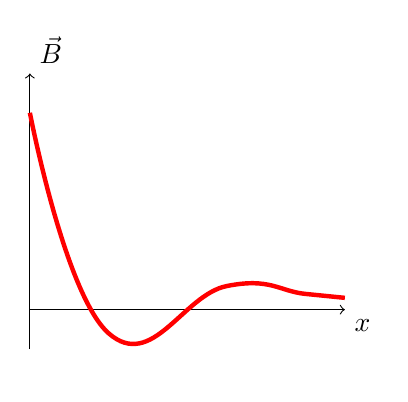
\begin{tikzpicture}
			%Achsen
			\draw[->](0,0)--(4,0)  node[below right]{$x$};
			\draw[->](0,-.5)--(0,3)node[above right]{$\vec{B}$};
				\draw[red,ultra thick] plot[smooth, tension=.8] coordinates {(0,2.5)(1,-0.3)(2.5,0.3)(3.5,0.2)(4,0.15)};
			\end{tikzpicture}
		}
}
	\caption{Leiter in $z$-Richtung}
\end{wrapfigure}

Ein Beispiel für dieses Verhalten von Feldern und Strömen in Leitern ist die Entstehung von Wirbelströmen in von einem Magnetfeld durchsetzten Eisenkern. Dieser fungiert als Abschirmstrom und verhindert somit das tiefe Durchdringen des Kerns durch das Magnetfeld. In technischen Anwendungen wie z.B. dem Transformator wird dem entgegengewirkt, indem die Leitfähigkeit $\sigma$ durch Lamellierung stark abgesenkt wird.\\
\ \\ \linebreak

\begin{wrapfigure}[]{r}[0cm]{0cm}
	\raisebox{0pt}[\dimexpr\height-1\baselineskip\relax]{
		\colorbox{hgrey}{
			\begin{tikzpicture}
			%Achsen
			\draw (-1,-2)--(-1,2);
			\draw (1,-2)--(1,2);
			\draw[red, ultra thick, -latex] (0,1.8) [partial ellipse=60:430:.8cm and 0.2cm];
			\draw[red] (0,1.6)node[below right]{$\vec{B}$};
			\fill[pattern=north west lines] plot[smooth, tension=.8] coordinates {(0,-2)(.5,-1.5)(0.9,0)(1,-0.01)(1,-2)};
			\fill[pattern=north east lines] plot[smooth, tension=.8] coordinates {(0,-2)(-.5,-1.5)(-0.9,0)(-1,-0.01)(-1,-2)};
			\draw plot[smooth, tension=.8] coordinates {(0,-2)(-.5,-1.5)(-0.9,-0.01)(-1,0.3)};
			\draw (1.3,-1) node{$\vec{j}$};
			\draw plot[smooth, tension=.8] coordinates {(0,-2)(.5,-1.5)(0.9,-0.01)(1,0.3)};
			\draw (1.3,-1) node{$\vec{j}$};
			\draw[->] (-1.3,-1.5)-- node[left]{$\vec{E}$}(-1.3,-0.5);
			\end{tikzpicture}
		}
	}
	\caption{Skin-Effekt im Leiter}
\end{wrapfigure}

Ein anderes Beispiel ist der sogenannte \textbf{Skin-Effekt}, welcher dafür sorgt, dass Wechselströme an der Drahtoberfläche fließen. Der Widerstand eines Drahtes bei Skin-Effekt lässt sich folgendermaßen berechnen:

\begin{equation*}
Z \ = \ \frac{U}{I} \ = \ \frac{E \cdot l}{I} \quad \Rightarrow \quad \frac{Z}{l} \ = \ \frac{E}{I}
\end{equation*}

$E$ ist dabei ein von außen angelegtes elektrisches Feld. Weiterhin nehmen wir an, dass ein starker Skin-Effekt vorliegt $(\delta\ll r)$. Zunächst müssen wir also den Strom $I$ berechnen, um den Widerstand zu erhalten:


\begin{align*}
I  \ &= \ \Int{}{}{\vec{A}_F}\cdot\vec{j} \ = \ \sigma \ 2 \pi \ r \Int{0}{\infty}{x} E(x) \qquad\qquad\qquad\Big| \ E(x) = E\cdot e^{(i-1)k_0 x}\\
&= \ 2\pi \sigma \ E \ r \Int{0}{\infty}{x}e^{(i-1)k_0 x}  \ = \ 2\pi\sigma \ E \ r  \frac{1}{(i-1)k_0}\cdot(-1) 
\end{align*}

\newpage
Somit erhalten wir für den Widerstand:

\begin{equation*}
\frac{Z}{l}  \ = \ \frac{(1-i)k_0}{2\pi\sigma \ r} \ = \ \frac{1-i}{2\pi \ r}\ \sqrt{\frac{\mu\omega}{2\sigma}}
\end{equation*}

Vergleicht man dies mit dem normalen \textsc{Ohm}'schen Widerstand eines Leiters, so stellt man fest, dass der Widerstand bei Skin-Effekt sehr viel größer als dieser ist:

\begin{equation*}
\frac{R}{l} \ = \ \frac{1}{\pi \ r^2 \ \sigma} \quad \Rightarrow \quad \frac{Z}{R}  \ = \ \frac{1-i}{2} \ \frac{r}{\delta} \ \gg \ 1
\end{equation*}
